\clearpage
\section{TR-Bedienung}
Diese Anleitung ist für den \textbf{TI-Nspire CX CAS} Rechner.\\[0.4cm]
\begin{tabular}{ll}
	Matrizen \& Vektoren einfügen: & 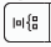
\includegraphics[height=0.6cm]{pics/TR_Symbol.png} $\rightarrow$ gewünschtes Element auswählen\\[0.2cm]
	Zeile an Matrix hinzufügen: & 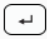
\includegraphics[height=0.6cm]{pics/TR_Enter_Pfeil.png}\\[0.2cm]
	Spalte an Matrix hinzufügen: & 
\includegraphics[height=0.6cm]{pics/TR_Shift.png} $\rightarrow$ 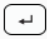
\includegraphics[height=0.6cm]{pics/TR_Enter_Pfeil.png}\\[0.8cm]
	
	Determinante: & det($[...]$) $\rightarrow$ 
\includegraphics[height=0.6cm]{pics/TR_Enter.png}\\[0.2cm]
	& oder\\[0.2cm]
	& 
\includegraphics[height=0.6cm]{pics/TR_Menu.png} $\rightarrow$ 7 $\rightarrow$ 3 $\rightarrow$ 
\includegraphics[height=0.6cm]{pics/TR_Enter.png}\\[0.2cm]
	Inverse: & $[...]^{-1} \rightarrow$ 
\includegraphics[height=0.6cm]{pics/TR_Enter.png}\\[0.2cm]
	Transponieren & $[...]$ 
\includegraphics[height=0.6cm]{pics/TR_Menu.png} $\rightarrow$ 7 $\rightarrow$ 2 $\rightarrow$ 
\includegraphics[height=0.6cm]{pics/TR_Enter.png}\\[0.2cm]
	Gauss ohne rückw. einsetzen: & ref($[...]$) $\rightarrow$ 
\includegraphics[height=0.6cm]{pics/TR_Enter.png}\\[0.2cm]
	Gauss: & rref($[...]$) $\rightarrow$ 
\includegraphics[height=0.6cm]{pics/TR_Enter.png}\\[0.2cm]
	Gauss Schritte ohne Rückw.\footnotemark[1]: & linalgcas\textbackslash gausstep($[...]$) $\rightarrow$ 
\includegraphics[height=0.6cm]{pics/TR_Enter.png}\\[0.2cm]
	Inverse Schritte\footnotemark[1]: & linalgcas\textbackslash inversestep($[...]$) $\rightarrow$ 
\includegraphics[height=0.6cm]{pics/TR_Enter.png}\\[0.8cm]
	
	Kreuzprodukt: & crossP([X,Y,Z],[X,Y,Z])\\[0.2cm]
	Skalarprodukt: & dotP([X,Y,Z],[X,Y,Z])\\[0.2cm]
	Betrag: & norm([X, Y, Z])\\[0.8cm]
	
	Eigenwerte: & cPolyRoots($r^2 + 2r + 1$, $r$)\\[0.2cm]

\end{tabular}
\footnotetext[1]{Nur wenn LinAlgCAS Library vorhanden ist.}
